\documentclass[11pt,a4paper]{article}
\usepackage[english]{babel}
\usepackage[utf8]{inputenc}
\usepackage{verbatim}
\usepackage{amssymb}
\usepackage{graphicx}

\title{BW4T - Refactoring}

\date{\today}

\begin{document}

\maketitle

\section{Hoe het nu is}
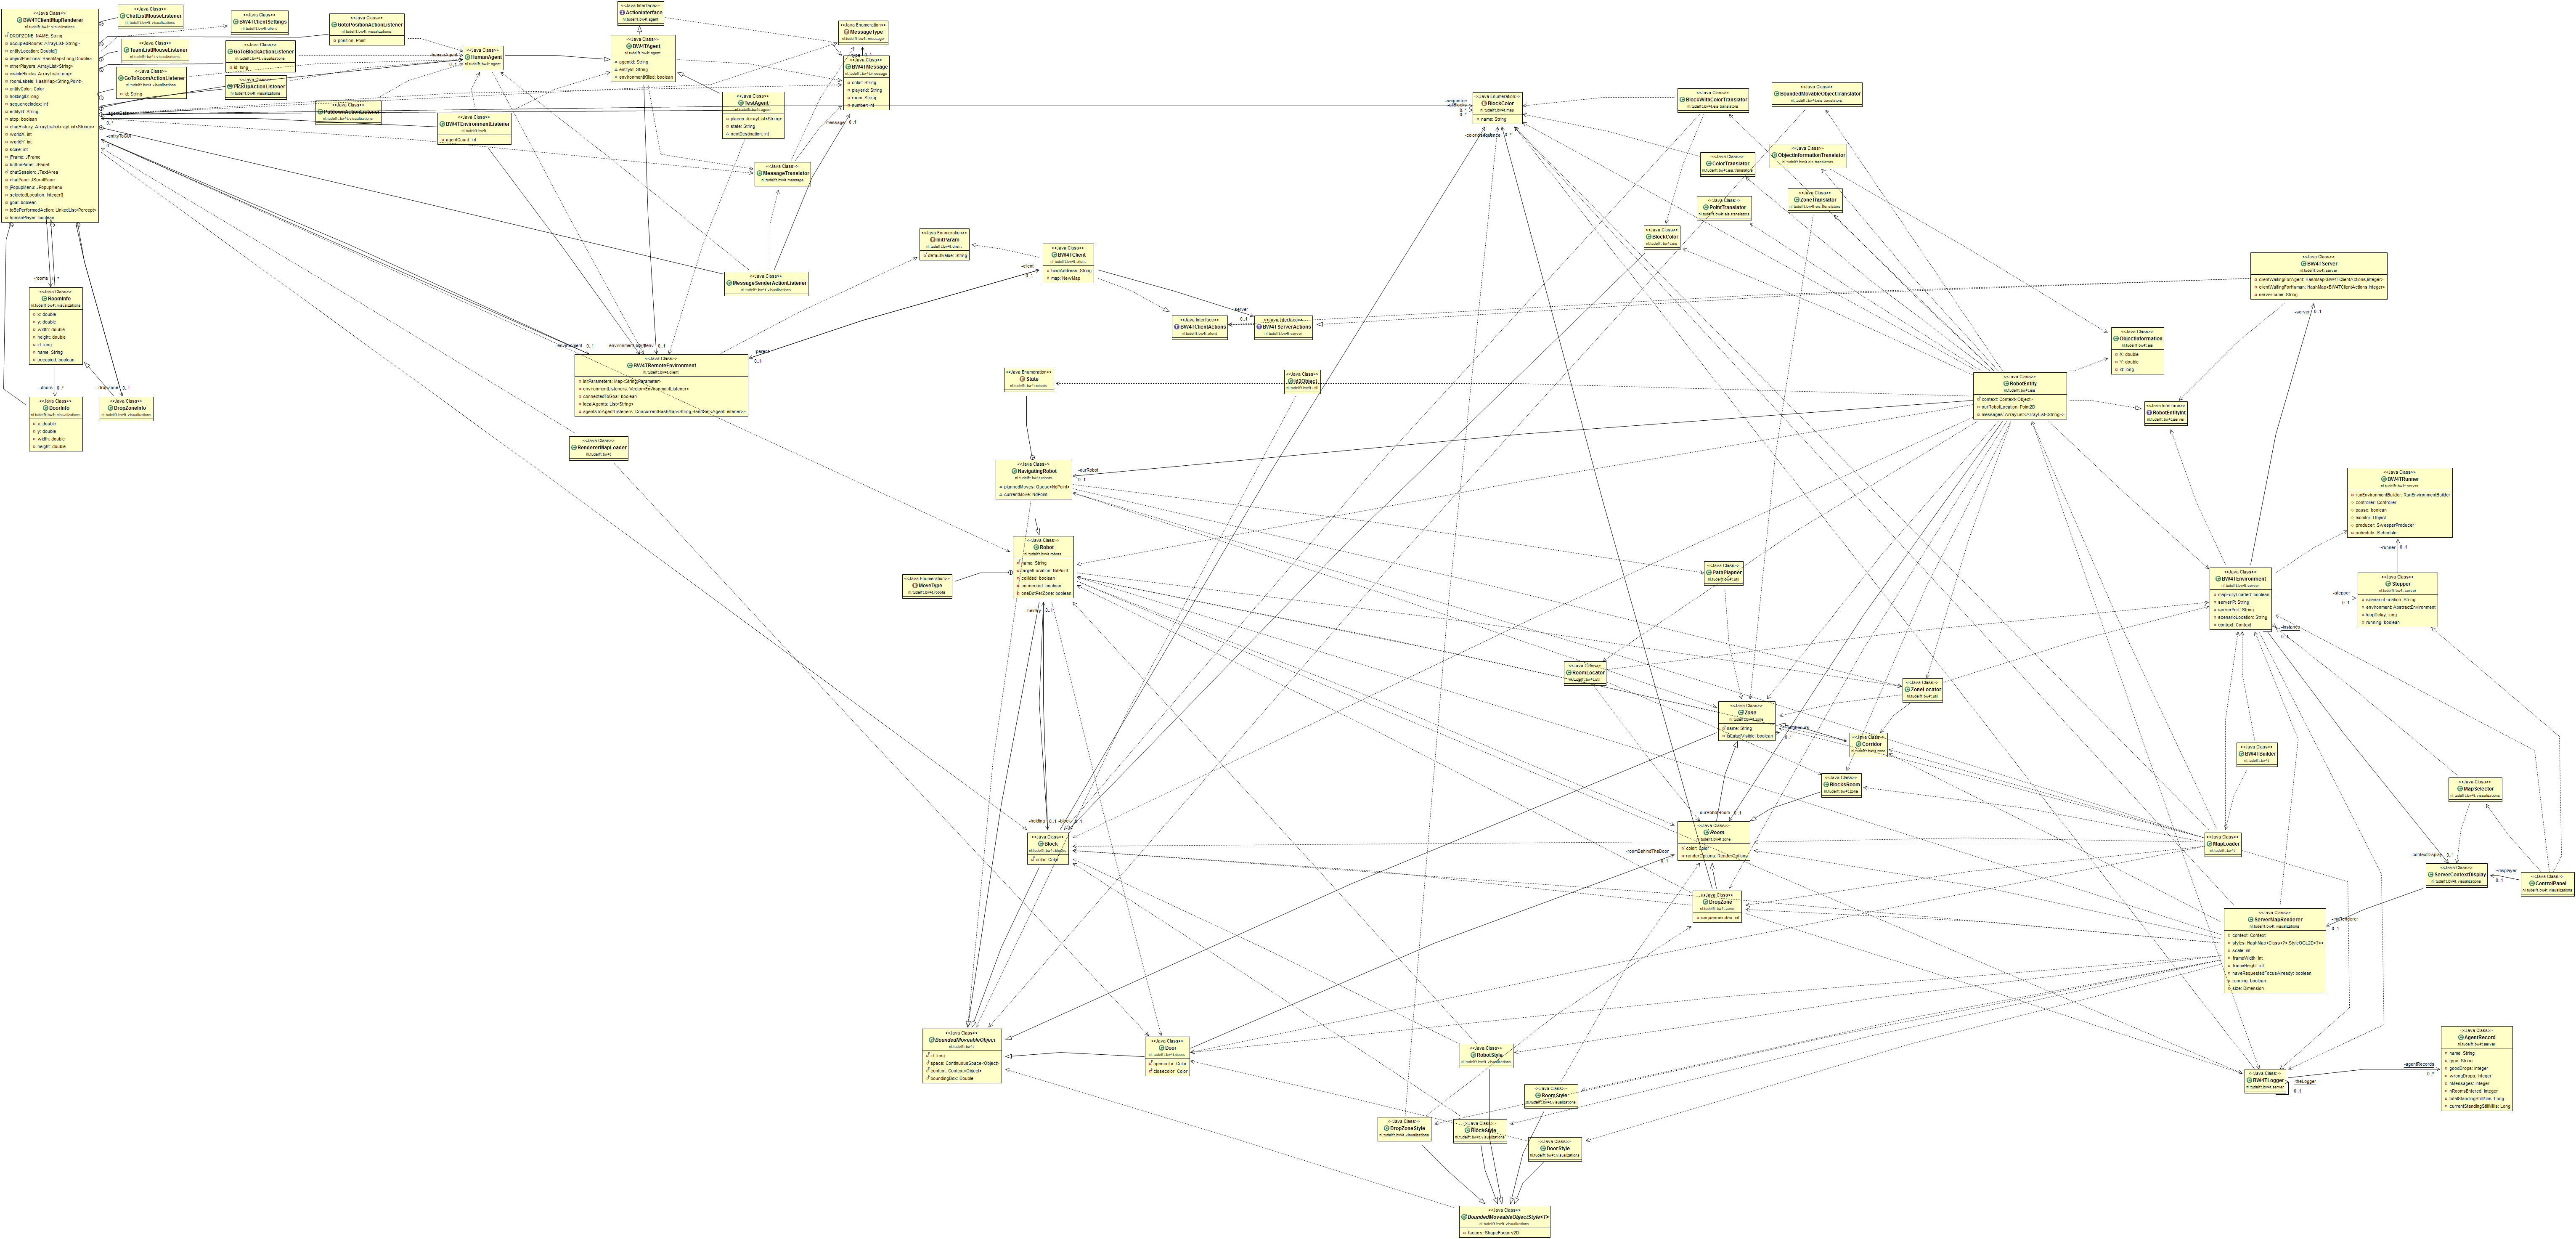
\includegraphics[width=\linewidth]{old.png}
Zoals in het UML diagram te zien is zijn veel klassen met elkaar verbonden. De documentatie is erg matig en er zijn geen testen. Deze factoren zorgen ervoor dat het heel lastig is om de code te begrijpen en te debuggen. Het is lastig uit te vinden wat een stukje code doet, wat de functie van een methode is, wat het verschil is tussen bepaalde methodes en klassen en wat de connectie is tussen stukken code. \\
In het huidige systeem zit Repast, maar veel functies die ook in Repast zitten worden apart geimplementeerd. Hier zorgt Repast ervoor dat de totale size van de systeem erg groot is (500 mb voor Repast alleen). \\
In het huidige systeem zit een client en server klasse, maar de client en server worden niet consistent gebruikt. De client en server zitten niet los van elkaar, en er zijn klassen die met elkaar communiceren buiten de client en server om terwijl ze dit niet zouden moeten doen bij een client-server architecture. \\
Het opstarten van het systeem is nu ook niet heel gebruiksvriendelijk, de client en server moeten apart opgestart worden. 
Zie ook bijlage voor voorbeelden van 'slechte' code en comments.

\section{Wat hebben we tot nu toe bereikt}
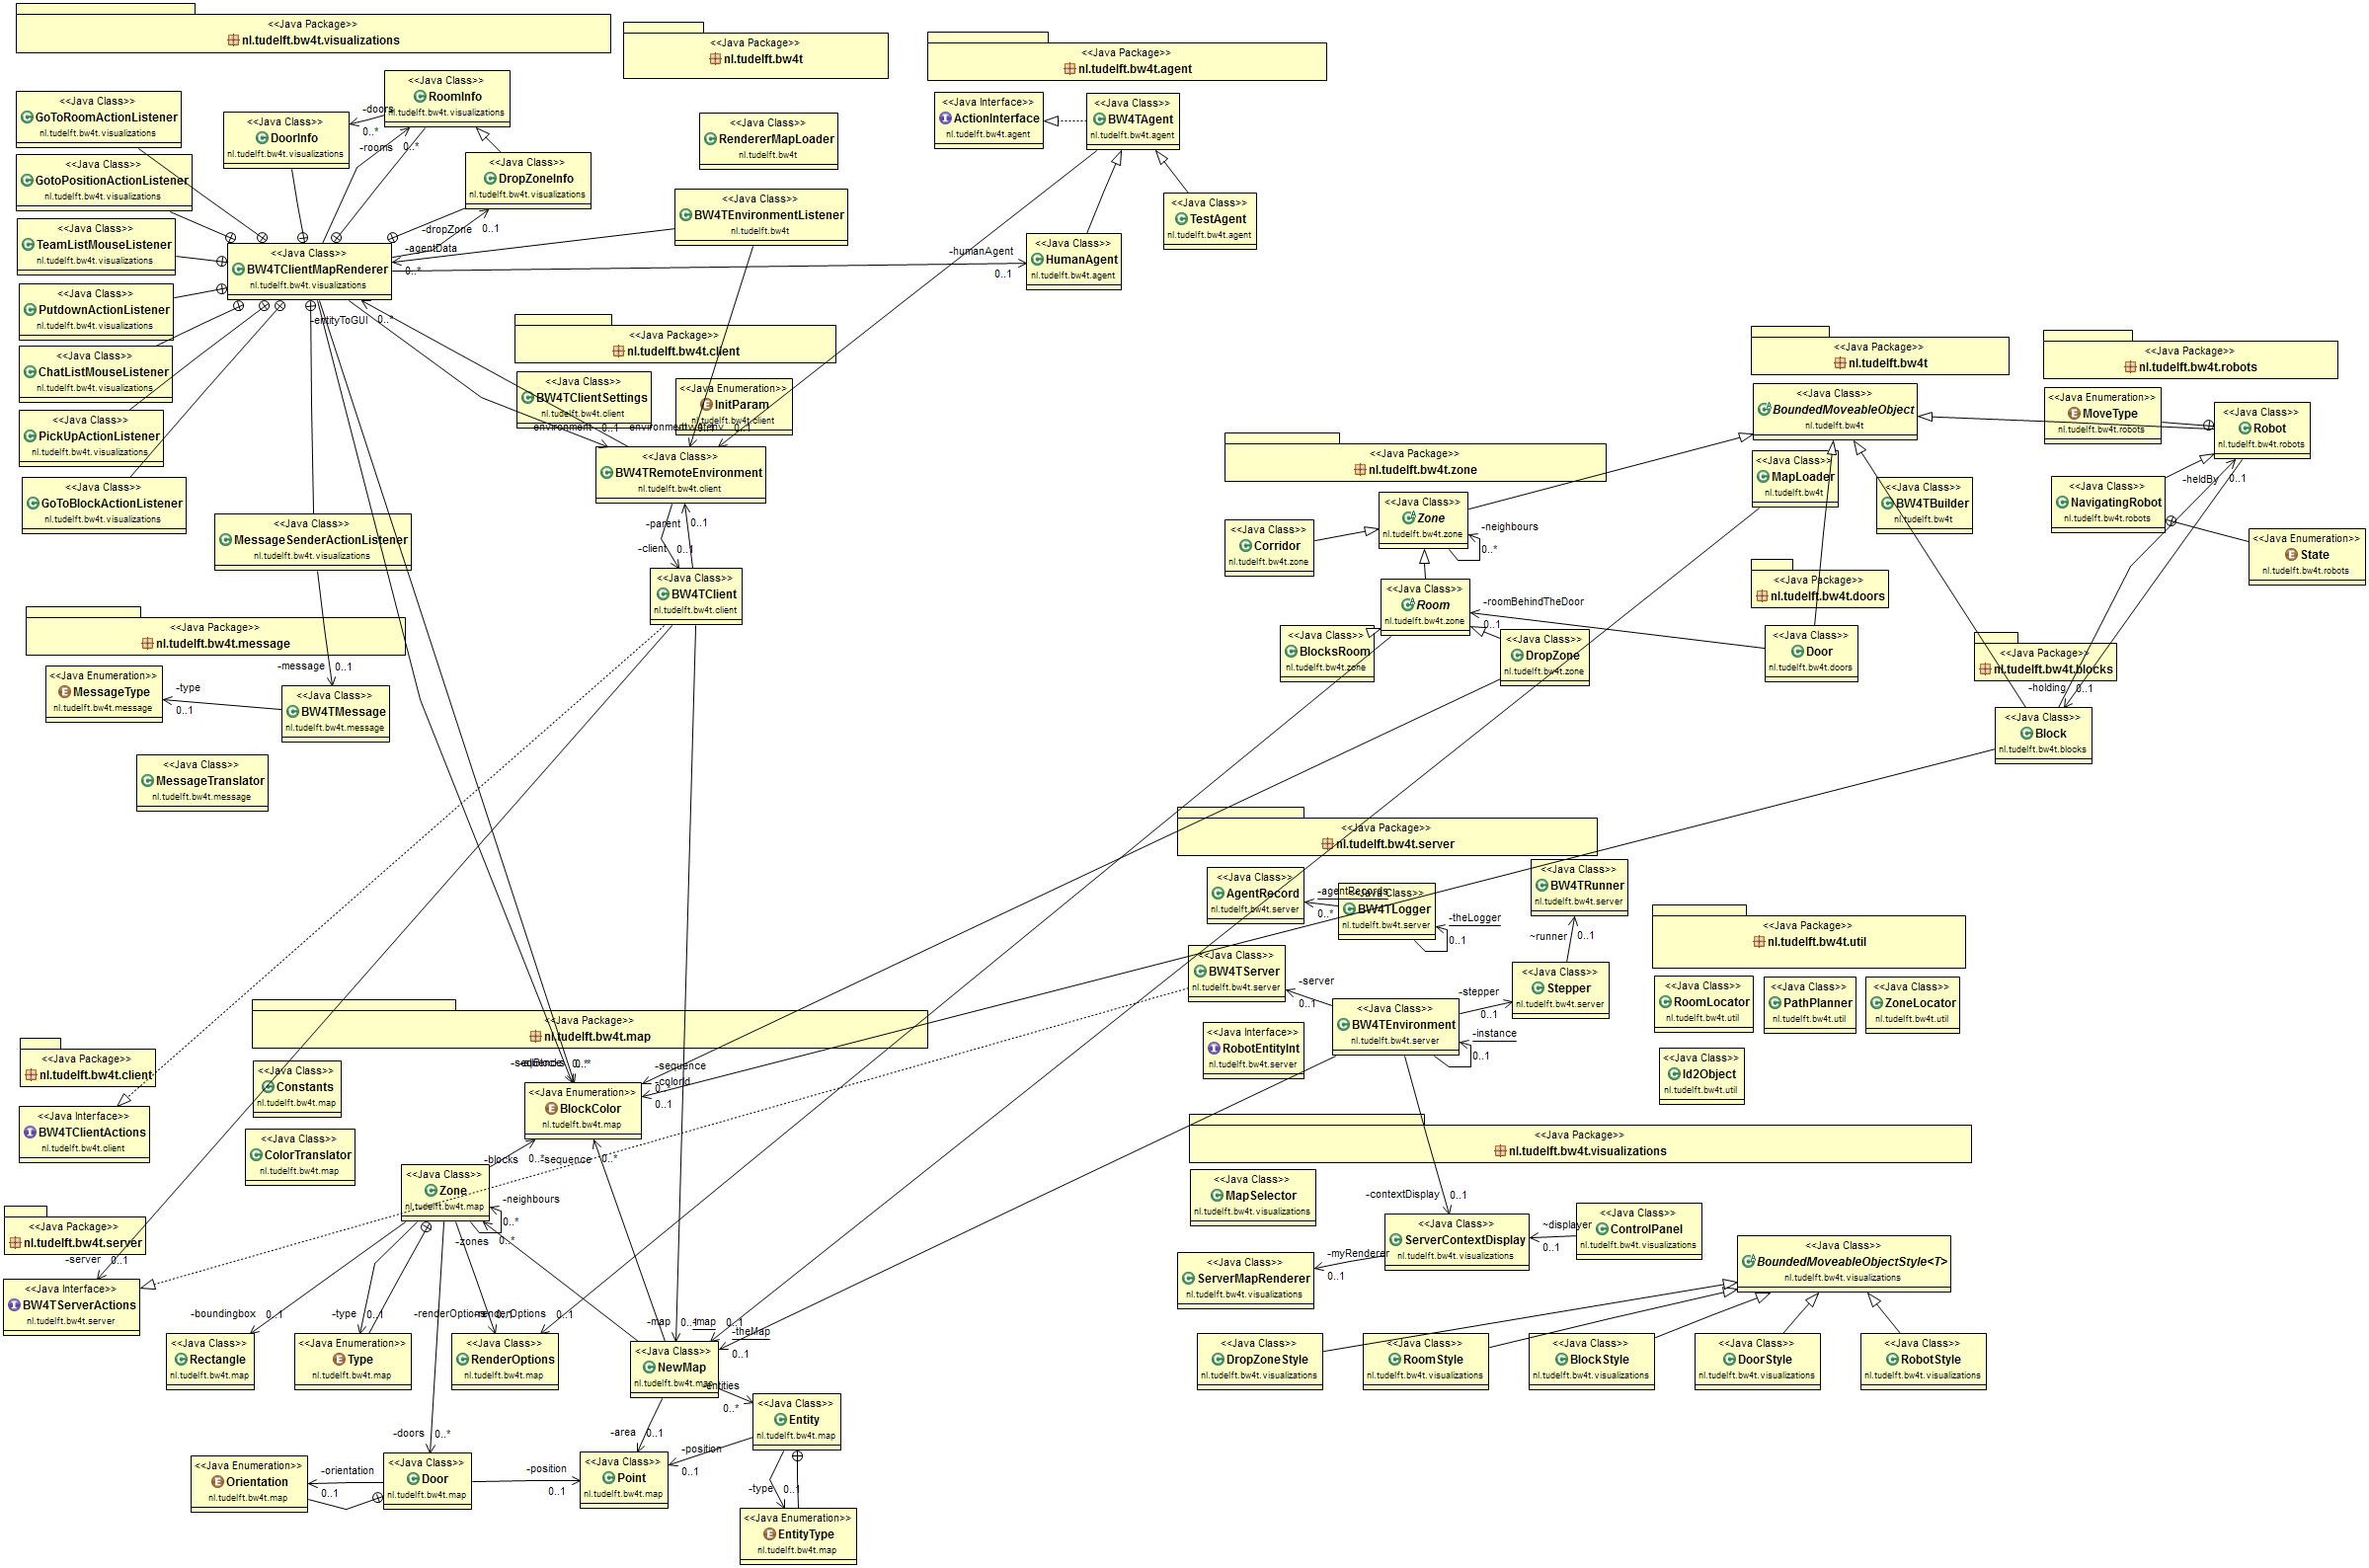
\includegraphics[width=\linewidth]{UMLv2.png}
Repast is nu een plugin en de bijbehorende jar files zijn uit het systeem, wat veel minder ruimte kost (nu nog maar 8mb). De plugin is de nieuwste versie van Repast. \\
We zijn bezig geweest met het splitsen van de server, client en een core. In core zitten de klassen die zowel door de server en de client gebruikt wordt. Elk van deze onderdelen is nu een apart Maven project. Met deze structuur hopen wij meer overzicht te krijgen in de code en dat het voor andere mensen ook (snel) duidelijk is hoe het systeem in elkaar zit. Verder is het testen van het systeem met deze structuur een stuk makkelijker. 

\section{Repast}
Repast is zeker een goed platform voor agent-based modeling. Echter voor dit project zullen we geen verder gebruik maken Repast dan hoe het nu gebruikt wordt. Dit omdat we problemen verwachten als we Repast meer gaan gebruiken. Met name het synchroon lopen met GOAL is een uitdaging. Als we het systeem meer gebruik willen laten maken van Repast zal er een hoop moeten worden omgeschreven. Wij zijn niet in staat dit in 5 weken te doen, aangezien we zoveel moeten veranderen dat er dan geen werkend product is. \\

\section{Wat kunnen wij aankomende weken nog bereiken}
Wat wij de aankomende weken nog kunnen doen is zorgen dat het opstarten van het systeem makkelijker is. Dus dat de server en client niet apart opgestart hoeven te worden, maar dat er een launcher is die alles voor je doet. \\
Ook zullen we de client-server architecture verder uitwerken. Hierbij willen we proberen om het systeem te versimpelen door overbodige connecties tussen klasses te verwijderen of om te zetten naar client-server communicatie. Ook zullen we de documentatie van het systeem proberen te verbeteren. \\
Een ander punt waar we aan gaan werken is het schrijven van testen. Dit zullen voornamelijk functionaliteitstesten zijn. \\
In de bijlage bevindt zich ook de toepassing van de MoSCoW-methode.

\section{Wat zou er kunnen gebeuren}
Als we meer tijd en ervaring zouden hebben zouden we het hele systeem omgooien. Zodanig dat de server-client architecture nog beter wordt geimplementeerd, de documentatie duidelijk is, en alles in het systeem goed getest is. Bij een langer lopend project is het te overwegen om alsnog Repast te gaan gebruiken. Dit zou dus betekenen dat er ook goed naar de link tussen GOAL en Repast gekeken moet worden. \\
Het is dan ook heel belangrijk dat het overzicht bewaart blijft, dat er kritisch naar de code wordt gekeken zodat het systeem optimaal werkt.

\newpage
\section*{Bijlagen} 
Deze bijlage bevat een aantal voorbeelden van 'slechte' code en comments. Het zijn situaties die we willen verbeteren en voorkomen. \\

Lege methodes \\
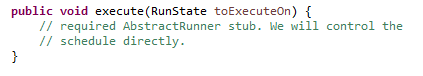
\includegraphics[width=\linewidth]{emptyMethod.png} \\ 

Twee methodes die op elkaar lijken maar niet duidelijk het verschil wordt aangegeven. \\
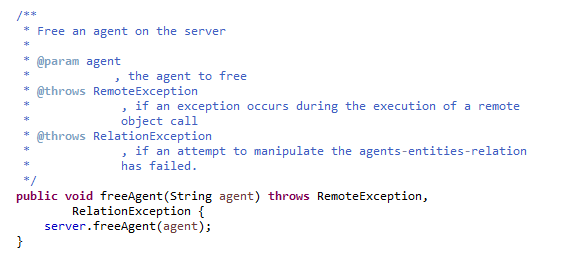
\includegraphics[width=\linewidth]{freeAgentNoClue.png}
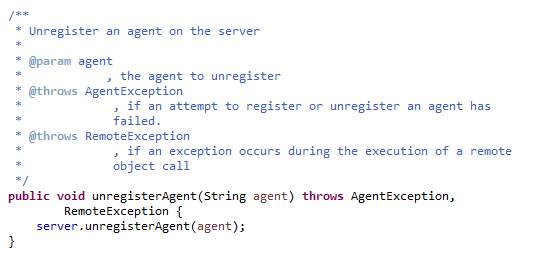
\includegraphics[width=\linewidth]{unregisterAgentNoClue.png} \\ 

Hacks \\
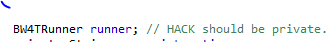
\includegraphics[width=\linewidth]{HackWTF.png} \\ 

Uitgecommende code, zeker bij een eindversie is het netter om dit eruit te halen \\
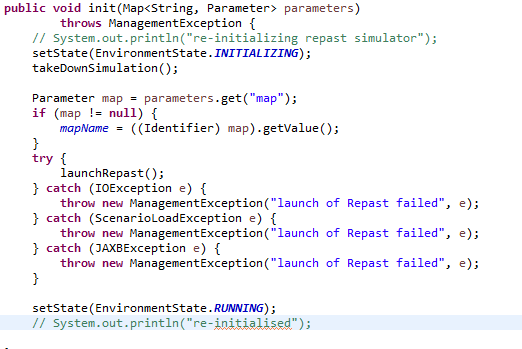
\includegraphics[width=\linewidth]{lelijkCode.png} \\ 

Er wordt niet gechecked of er inderdaad aan de voorwaarde wordt voldaan dat alle entities en agents ontbonden zijn\\
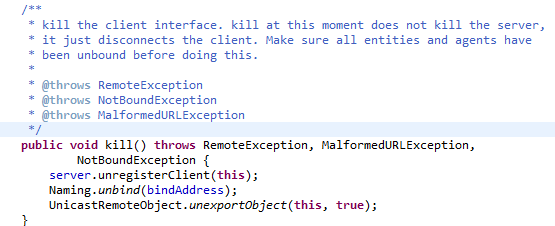
\includegraphics[width=\linewidth]{noEntityCheck.png} \\ 

Niet getest, op de gok iets proberen \\
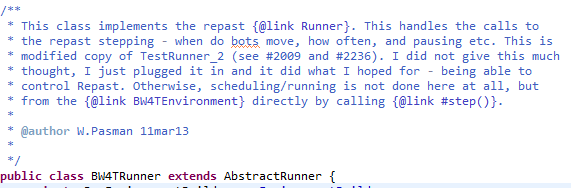
\includegraphics[width=\linewidth]{notTested.png} \\ 

Zou gedaan moeten worden, maar is dus niet gedaan \\
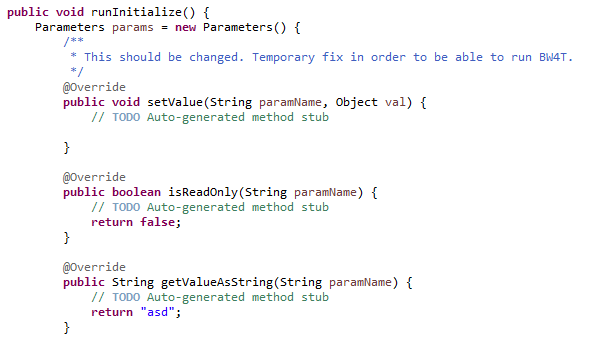
\includegraphics[width=\linewidth]{TODOs+shouldBeFixed} \\

\newpage
\section*{MoSCoW}
\subsection*{Must}
\begin{enumerate}
\item[-] Fully integration tests
\item[-] Test coverage of 50 $\%$
\item[-] System works same as before refactoring, functionallities are the same
\item[-] Documentation codeBase complete on package level
\item[-] Wouter must know how the new architecture is
\item[-] Launcher
\item[-] New logger fully integrated, old logger does not excist anymore
\item[-] Good graphical overview
\item[-] Make sure that the stakeholders get why we do what we do (eg with Repast)
\item[-] Integration with other groups
\item[-] System with Jenskins and Sonar on server TU Delft
\item[-] Exception handling
\end{enumerate}

\subsection*{Should}
\begin{enumerate}
\item[-] Reduce indicated mistakes given by Sonar
\item[-] Documentation codeBase for core complete on classe level
\item[-] Visualization package for Client en Server mergen
\end{enumerate}

\subsection*{Could}
\begin{enumerate}
\item[-] Documentation codeBase complete on classe level
\item[-] Analysing tool wich make use of the logger
\item[-] Use CodeCity on old on new system
\end{enumerate}

\subsection*{Won't}
\begin{enumerate}
\item[-] Logger replay function
\item[-] More use of Repast
\item[-] Documentation codeBase complete on method level
\end{enumerate}


\end{document}
